\begin{itemize}
    \item Goal -- select hyper-parameter setup of GNN for a given task
    \item Evaluation -- obtained mean true GNN performance based on training set size
    \item Procedure -- fit again the regression model on training set and predict the performance on test set
\end{itemize}
\begin{columns}
\begin{column}{0.4\linewidth} 
\scalebox{0.4}{
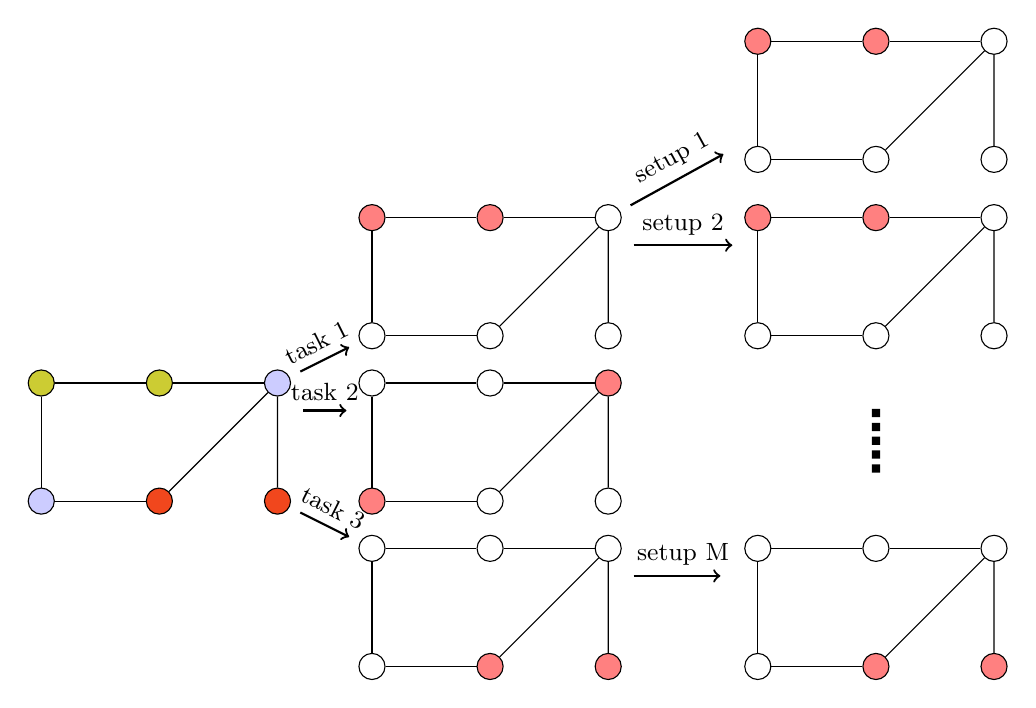
\begin{tikzpicture}[scale=0.7]
\def\dist{1.5cm}
\tikzset{node distance=\dist, minimum size=1ex}
	\tikzset{classA/.style={circle, draw=black, fill=blue!20!yellow}}
	\tikzset{classB/.style={circle, draw=black, fill=blue!20}}
	\tikzset{classC/.style={circle, draw=black, fill=yellow!20!red}}
	\tikzset{class1/.style={circle, draw=black, fill=red!50}}
	\tikzset{class0/.style={circle, draw=black, fill=white}}
	\tikzset{desc/.style={rectangle, anchor=west, text width=2.5cm,minimum height=1cm,minimum width=2.8cm, rounded corners=1ex, align=center}}

	\newcommand{\drawgraph}[9]{
\begin{scope}[xshift=#1, yshift=#2]
\node[#3] (#9A1) {};
\node[#4, right of=#9A1] (#9A2) {};
\node[#5, below of=#9A1] (#9B1) {};
\node[#6, right of=#9A2] (#9B2) {};
\node[#7, below of=#9A2] (#9C1) {};
\node[#8, below of=#9B2] (#9C2) {};
\draw [-] (#9A1) -- (#9A2);
\draw [-] (#9A1) -- (#9B1);
\draw [-] (#9B1) -- (#9C1);
\draw [-] (#9C1) -- (#9B2);
\draw [-] (#9B2) -- (#9C2);
\draw [-] (#9A2) -- (#9B2);
\end{scope}
	}

\drawgraph{0cm}{0cm}{classA}{classA}{classB}{classB}{classC}{classC}{base}
\drawgraph{6cm}{3cm}{class1}{class1}{class0}{class0}{class0}{class0}{task1}
\drawgraph{6cm}{0cm}{class0}{class0}{class1}{class1}{class0}{class0}{task2}
\drawgraph{6cm}{-3cm}{class0}{class0}{class0}{class0}{class1}{class1}{task3}
\drawgraph{13cm}{6.2cm}{class1}{class1}{class0}{class0}{class0}{class0}{task1par1}
\drawgraph{13cm}{3cm}{class1}{class1}{class0}{class0}{class0}{class0}{task1par2}
\drawgraph{13cm}{-3cm}{class0}{class0}{class0}{class0}{class1}{class1}{task3parN}
\draw[->, thick, shorten >=1ex, shorten <=1ex] (baseB2) -- (task1B1) node [pos=0.5, above, sloped] {\small{task 1}};
\draw[->, thick, shorten >=1ex, shorten <=1ex] ([yshift=-0.5cm] baseB2.east) -- ([yshift=-0.5cm] task2A1.west) node [pos=0.5, above, sloped] {\small{task 2}};
\draw[->, thick, shorten >=1ex, shorten <=1ex] (baseC2) -- (task3A1) node [pos=0.5, above, sloped] {\small{task 3}};
\draw[->, thick, shorten >=2ex, shorten <=1ex] (task1B2) -- ([yshift=2ex] task1par1B1.west) node [pos=0.5, above, sloped] {\small{setup 1}};
\draw[->, thick, shorten >=1ex, shorten <=1ex] ([yshift=-0.5cm] task1B2.east) -- ([yshift=-0.5cm] task1par2A1.west) node [pos=0.5, above, sloped] {\small{setup 2}};
\draw[->, thick, shorten >=2ex, shorten <=1ex] ([yshift=-0.5cm] task3B2.east) -- ([yshift=-0.5cm] task3parNA1.west) node [pos=0.5, above, sloped] {\small{setup M}};

\draw[dotted, line width=3pt, shorten >=5ex, shorten <=5ex] (task1par2C1) -- (task3parNA2);

\end{tikzpicture}}
    \end{column}

    \begin{column}{0.6\linewidth}
           \scalebox{0.55}{
    \begin{tabular}{p{2cm}p{4.3cm}p{5cm}}
        \toprule
        Method Name  & required GNN runs &  Procedure Description \\
        \midrule
        Optimal & All data-points & The best setup for given  task over all setups. \\ 
        Best Hyper-Parameter & All data-points & The setup with the best average performance over tasks for given data set. \\    
        Reference & Train set & Setup with the true best performance on training set + 1 random sample on testing set.\\
        Ours & Train set &  As reference with the best predicted performance on testing set instead of the random one.\\
        Ours -- cross-datasets & Train set + data-points from all datasets excepting the investigated one &  As in ours, but the model is trained also on other datasets.\\
        \bottomrule
    \end{tabular}
    } 
    \end{column}


\end{columns}
